\subsubsection{Proceso: Recomendar atributos contra un oponente}

\begin{itemize}
	\item \textbf{O1:} Busca las partidas jugadas por un jugador dado el nombre del juego y
		el nombre del jugador.\\

	\item \textbf{O2:} Busca los valores, en las patridas obtenidas
		en O1, de varios atributos dados sus nombres.\\
\end{itemize}

\begin{figure}[h!]
	\centering
	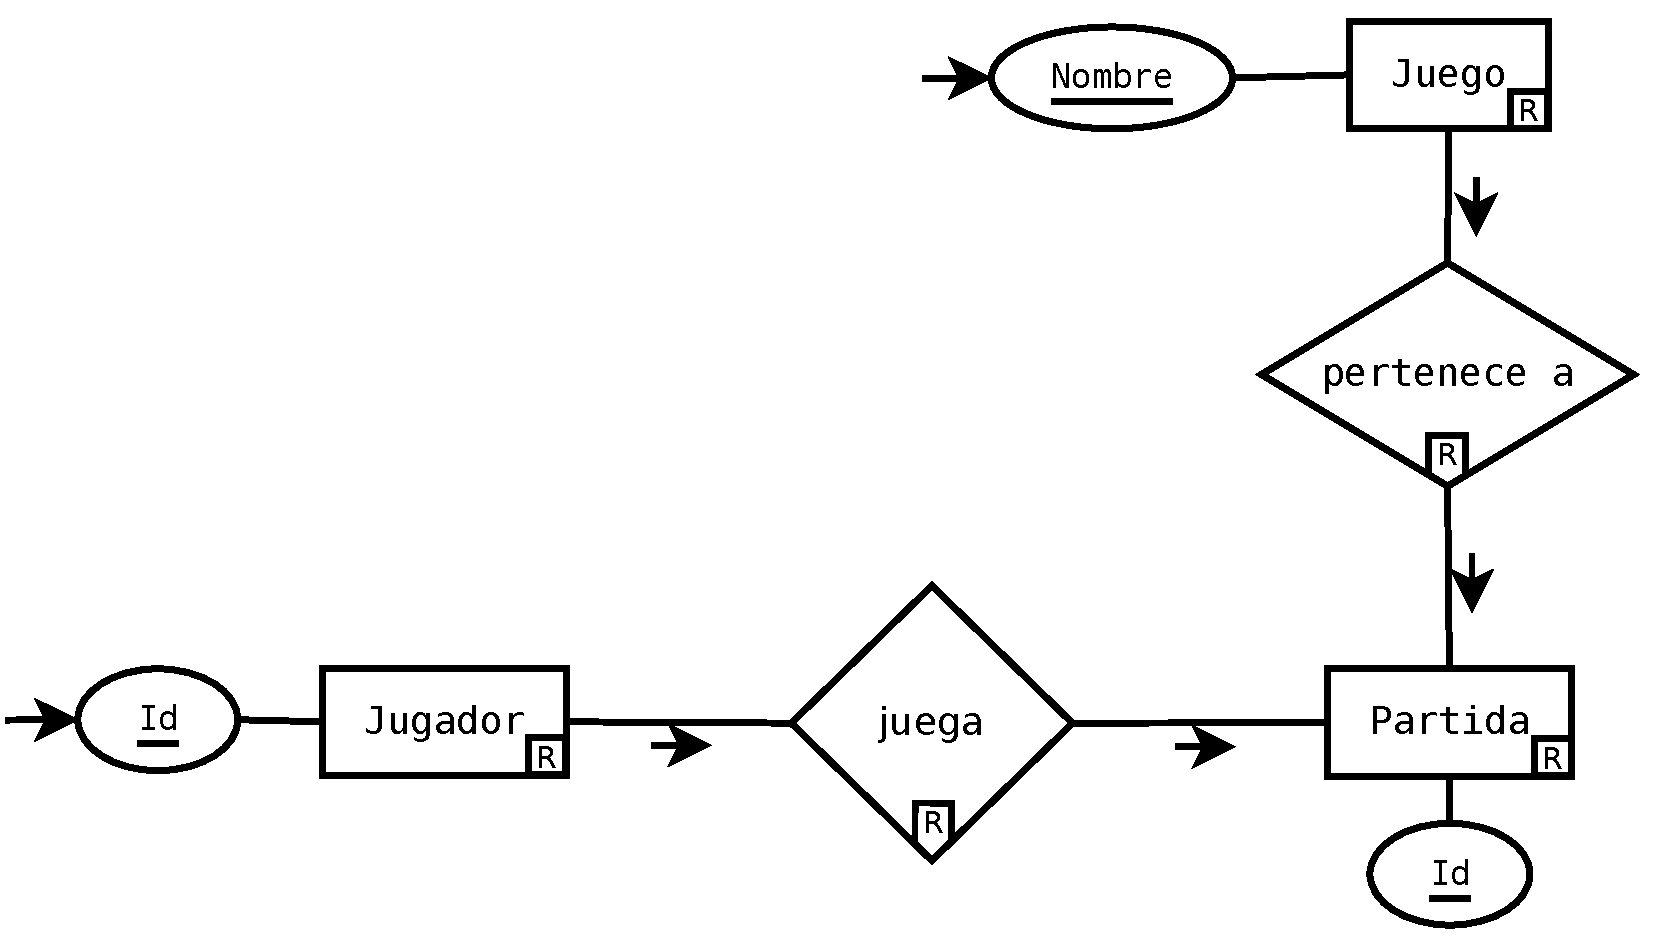
\includegraphics[width=0.5\linewidth]{../Diagramas/pdf/Op1-1.pdf}
	\caption{Esquema de navegabilidad de O1 del proceso 1}
\end{figure}

\begin{figure}[h!]
	\centering
	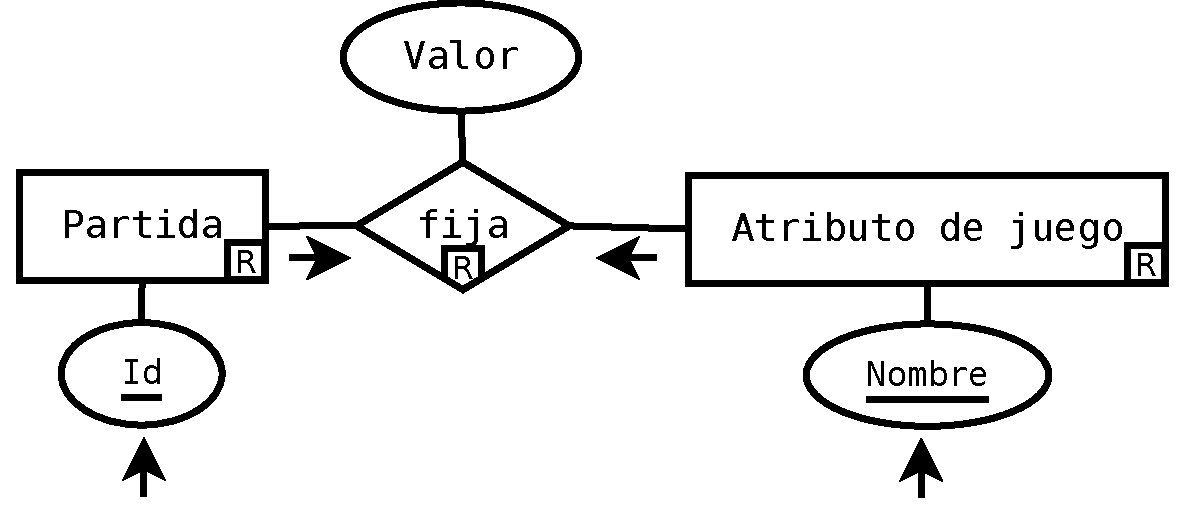
\includegraphics[width=0.5\linewidth]{../Diagramas/pdf/Op1-2.pdf}
	\caption{Esquema de navegabilidad de O2 del proceso 1}
\end{figure}



\subsubsection{Proceso: Recomendar estilo de juego parecido al de un jugador}

\begin{itemize}
	\item \textbf{O1:} Busca las partidas jugadas por un jugador dado el nombre del juego y
		el nombre del jugador.\\
	\item \textbf{O2:} Busca los valores, en las patridas obtenidas
		en O1, de varios atributos dados sus nombres.\\
\end{itemize}

\begin{figure}[h!]
	\centering
	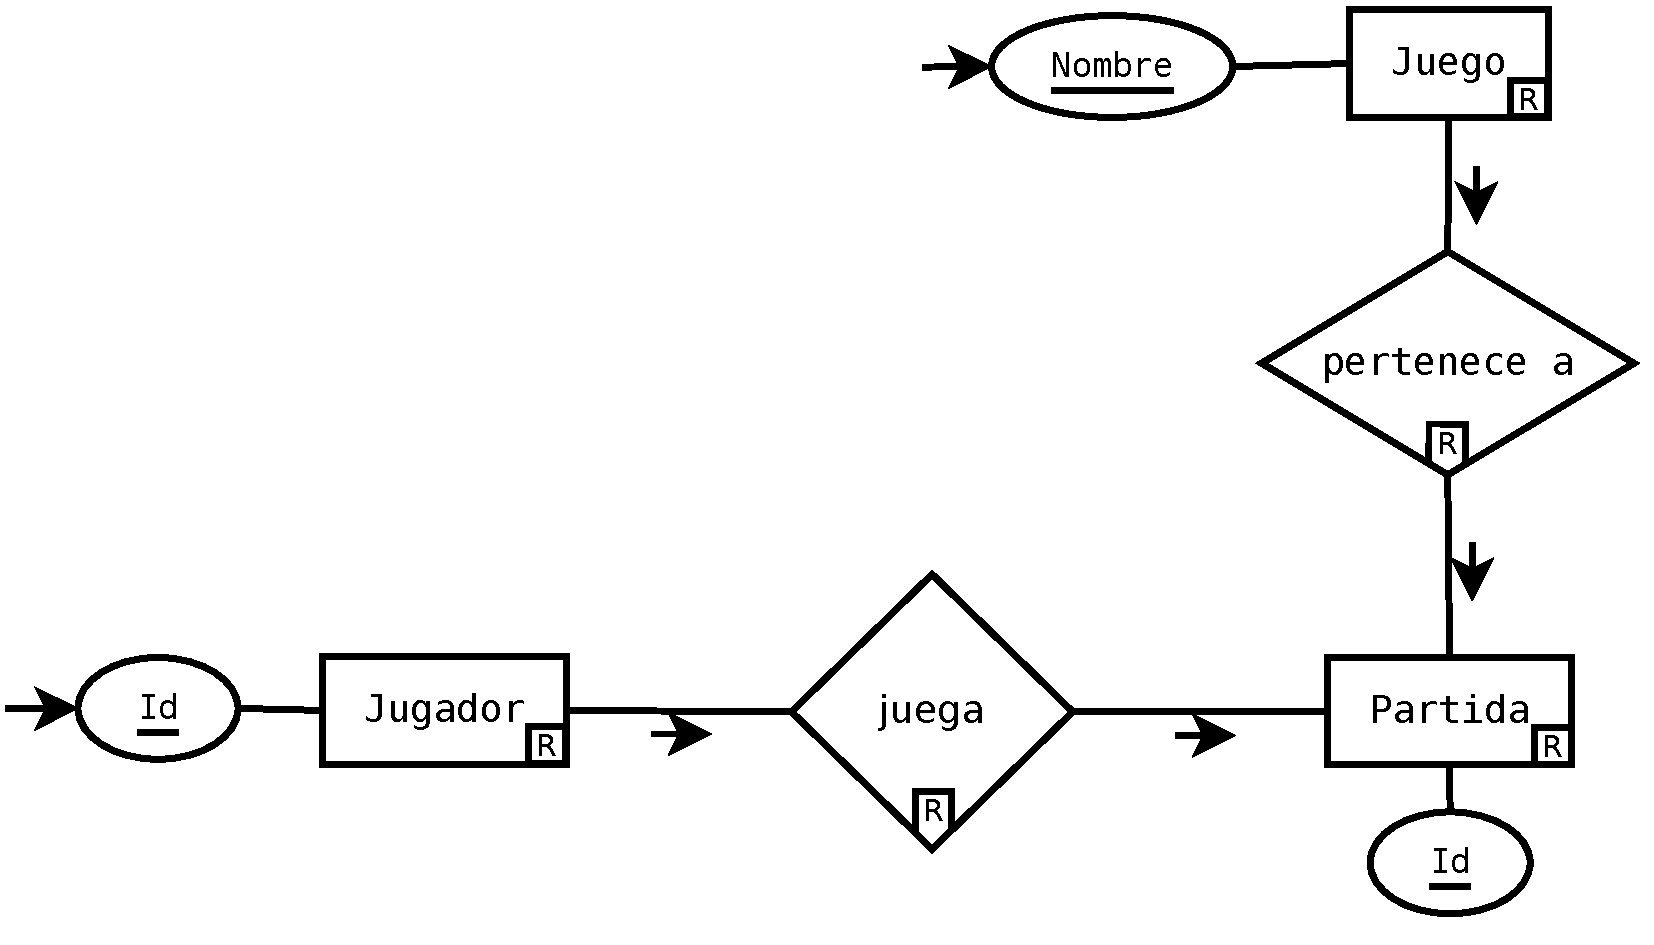
\includegraphics[width=0.5\linewidth]{../Diagramas/pdf/Op2-1.pdf}
	\caption{Esquema de navegabilidad de O1 del proceso 2}
\end{figure}

\begin{figure}[h!]
	\centering
	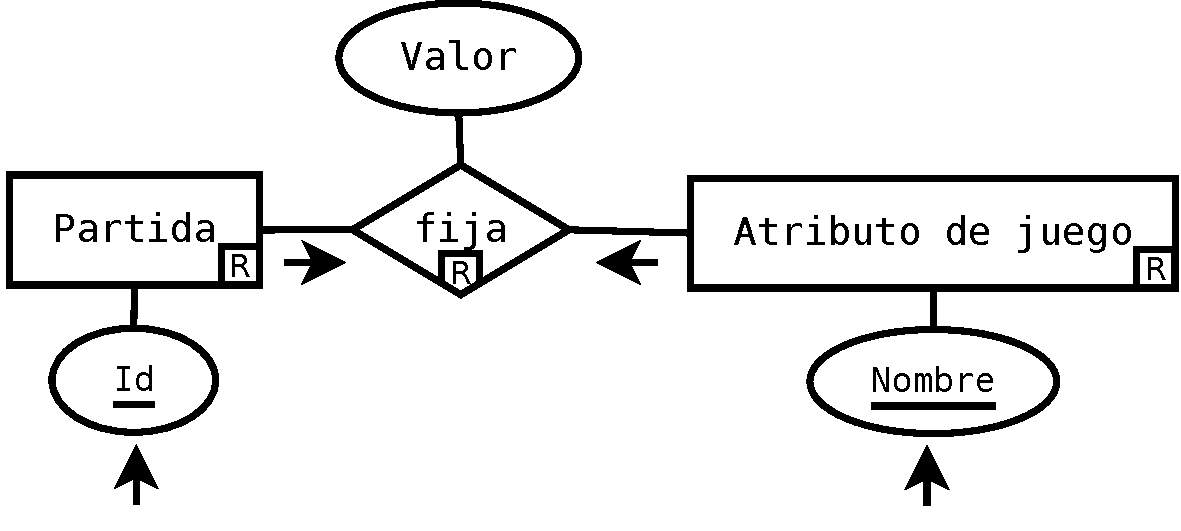
\includegraphics[width=0.5\linewidth]{../Diagramas/pdf/Op2-2.pdf}
	\caption{Esquema de navegabilidad de O2 del proceso 2}
\end{figure}



\subsubsection{Proceso: Recomendar atributos con contexto}

\begin{itemize}
	\item \textbf{O1:} Dado un nombre de juego y el nombre de varios
		atributos junto con un valor asociado a cada uno, 
		buscar las partidas en las que atributo y valor coincidan.\\
	\item \textbf{O2:} Dados varios nombres de atributos, buscar en las
		partidas obtenidas en O1 los valores correspondiantes a
		estos.\\
\end{itemize}

\begin{figure}[h!]
	\centering
	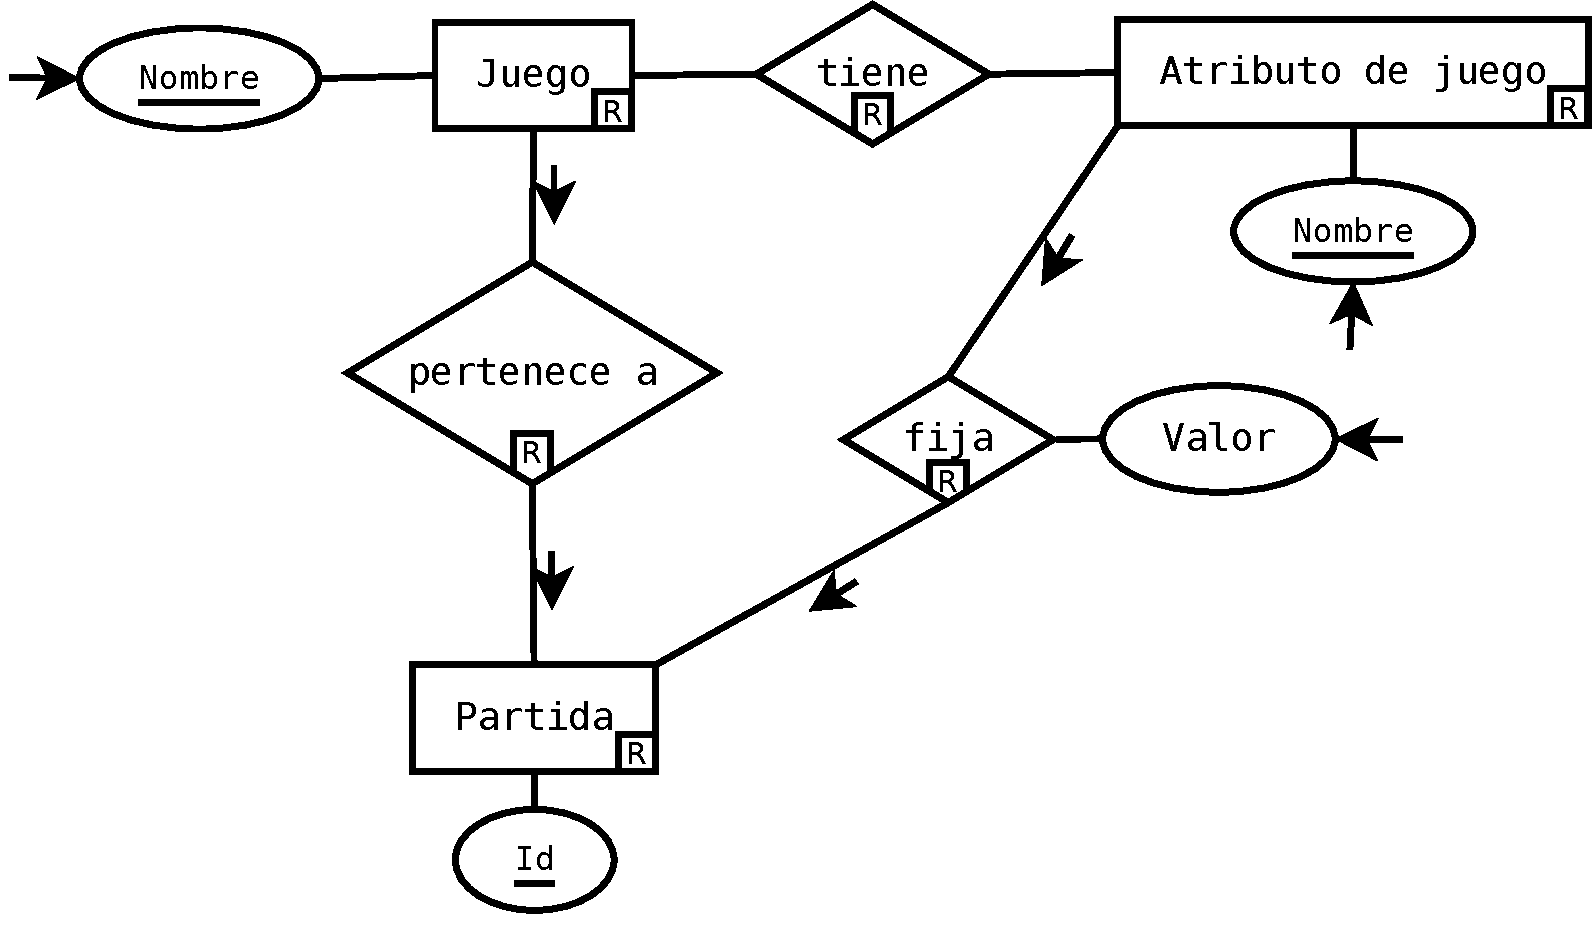
\includegraphics[width=0.5\linewidth]{../Diagramas/pdf/Op3-1.pdf}
	\caption{Esquema de navegabilidad de O1 del proceso 3}
\end{figure}

\begin{figure}[h!]
	\centering
	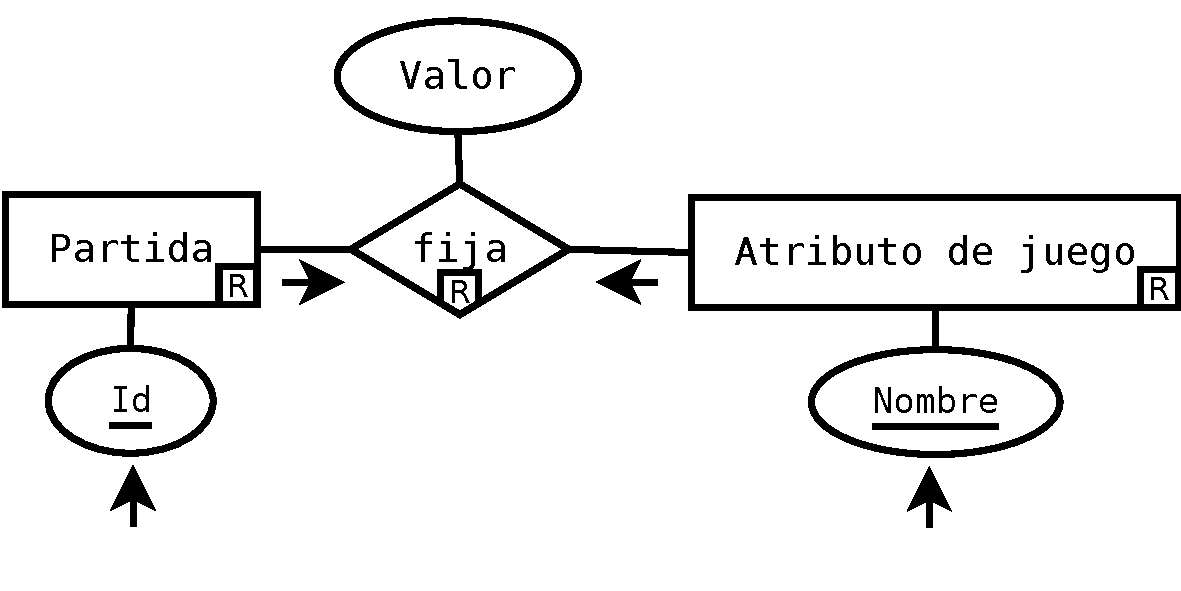
\includegraphics[width=0.5\linewidth]{../Diagramas/pdf/Op3-2.pdf}
	\caption{Esquema de navegabilidad de O2 del proceso 3}
\end{figure}



\subsubsection{Proceso: Recomendar atributos en general}

\begin{itemize}
	\item \textbf{O1:} Dado el nombre de un juego, el nombre de varios atributos y una puntuación
		, buscar los valores de los atributos anteriores en todas las partidas del juego
		que los contengan y cuya puntuación sea mayor que la dada, junto con la puntuación
		de esa partida.\\
\end{itemize}

\begin{figure}[h!]
	\centering
	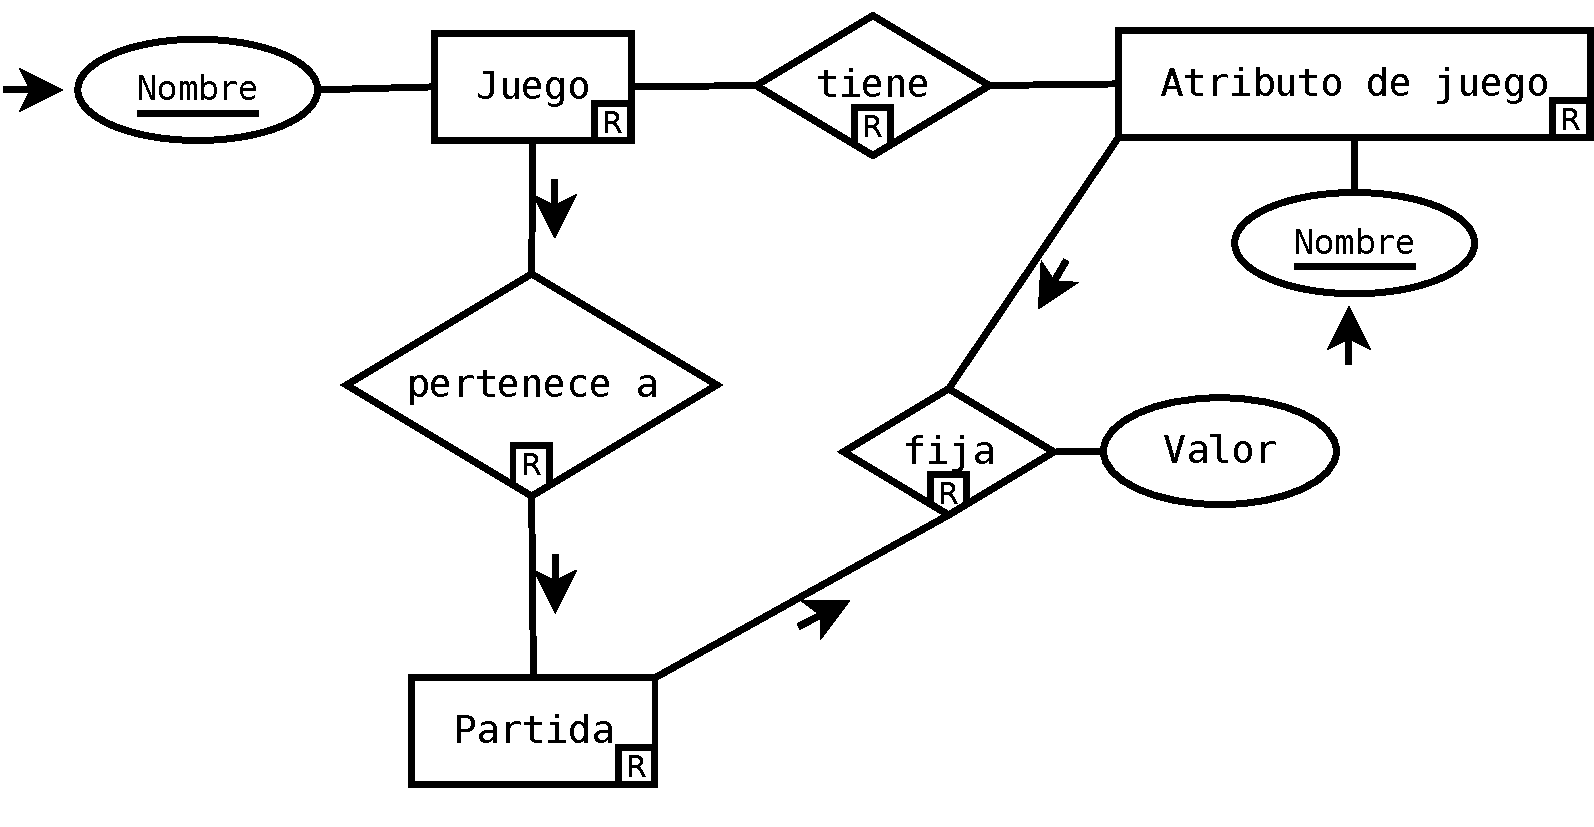
\includegraphics[width=0.5\linewidth]{../Diagramas/pdf/Op4-1.pdf}
	\caption{Esquema de navegabilidad de O1 del proceso 4}
\end{figure}

